\documentclass[12pt]{article}
\usepackage[margin=2.5cm]{geometry}
\usepackage{enumerate}
\usepackage{amsfonts}
\usepackage{amsmath}
\usepackage{fancyhdr}
\usepackage{amsmath}
\usepackage{amssymb}
\usepackage{amsthm}
\usepackage{mdframed}
\usepackage{graphicx}
\usepackage{subcaption}
\usepackage{adjustbox}
\usepackage{listings}
\usepackage{xcolor}
\usepackage{booktabs}
\usepackage[utf]{kotex}
\usepackage{hyperref}

\definecolor{codegreen}{rgb}{0,0.6,0}
\definecolor{codegray}{rgb}{0.5,0.5,0.5}
\definecolor{codepurple}{rgb}{0.58,0,0.82}
\definecolor{backcolour}{rgb}{0.95,0.95,0.92}

\lstdefinestyle{mystyle}{
    backgroundcolor=\color{backcolour},
    commentstyle=\color{codegreen},
    keywordstyle=\color{magenta},
    numberstyle=\tiny\color{codegray},
    stringstyle=\color{codepurple},
    basicstyle=\ttfamily\footnotesize,
    breakatwhitespace=false,
    breaklines=true,
    captionpos=b,
    keepspaces=true,
    numbers=left,
    numbersep=5pt,
    showspaces=false,
    showstringspaces=false,
    showtabs=false,
    tabsize=1
}

\lstset{style=mystyle}

\pagestyle{fancy}
\renewcommand{\headrulewidth}{0.4pt}
\lhead{CSC 343}
\rhead{Worksheet 3 Solution}

\begin{document}
\title{CSC343 Worksheet 3 Solution}
\maketitle

\bigskip

\begin{enumerate}[1.]
    \item \textbf{Exercise 6.1.1}:

    \bigskip

    If there is a comma between $A$ and $B$ (i.e, \textit{SELECT A, B}), we can
    conclude $A$ and $B$ are two different attributes.

    \bigskip

    If there are no commas between $A$ and $B$, we can conclude $B$ is an alias
    of $A$.

    \item \textbf{Exercise 6.1.2}:

    \begin{enumerate}[a)]
        \item SELECT address FROM Studio WHERE name = 'MGM';
        \item SELECT birthdate FROM MovieStar WHERE name = 'Sandra Bullock';
        \item SELECT starName FROM StarsIn WHERE movieYear = 1980, movieTitle LIKE '\%Love\%';

        \bigskip

        \begin{mdframed}
            \underline{\textbf{Correct Solution:}}

            \bigskip

            SELECT starName FROM StarsIn WHERE movieYear = 1980 \color{red}AND\color{black}\:movieTitle LIKE '\%Love\%';
        \end{mdframed}
        \item SELECT name FROM MovieExec WHERE netWorth $>=$ 10000000;
        \item SELECT name FROM MovieStar WHERE gender='male' OR address LIKE '\%Malibu\%';
    \end{enumerate}

    \item \textbf{Exercise 6.1.3}:

    \begin{enumerate}[a)]
        \item SELECT model, speed, hd FROM PC WHERE price $<$ 1000;
        \item SELECT model, speed AS gigahertz, hd AS gigabytes FROM PC WHERE price $<$ 1000;
        \item SELECT maker FROM Product WHERE type='printer';
        \item SELECT model, ram, screen FROM Laptops WHERE price $>$ 1500;
        \item SELECT * FROM Printer WHERE color=TRUE;
        \item SELECT model, hd FROM PC WHERE speed = 3.20 AND price $<$ 2000;
    \end{enumerate}


    \item \textbf{Exercise 6.1.4}:

    \begin{enumerate}[a)]
        \item SELECT class, country FROM Classes where numGuns $>=$ 10;
        \item SELECT name AS shipName FROM Ships WHERE launched $<$ 1918;
        \item SELECT ship, battle FROM Outcomes WHERE result='sunk';
        \item SELECT name FROM Ships WHERE name = class;
        \item SELECT name FROM Ships WHERE name LIKE 'R\%';
        \item SELECT name FROM ships WHERE name LIKE '\% \% \%';
    \end{enumerate}

    \item \textbf{Exercise 6.1.5}:
    \begin{enumerate}[a)]
        \item Given $a = 10$, the sets of tuples that satisfy the condition is

        \bigskip

        $(10, -MAX\_INT), (10,-MAX\_INT + 1), \cdots (10,0), \cdots, (10,MAX\_INT - 1), \\
        (10,MAX\_INT), (10, NULL)$

        \bigskip

        Given $b = 20$, the sets of tuples that satisfy the condition is

        \bigskip

        $(-MAX\_INT, 20), (-MAX\_INT + 1, 20), \cdots (0, 20), \cdots, (MAX\_INT - 1, 20), \\
        (MAX\_INT, 20), (NULL, 20)$

        \bigskip

        Given $a = 10$ and $b = 20$, the set of tuple that satisfy the condition
        is $(10, 20)$

        \item

        Given $a = 10$ AND $b = 20$, the only set of $(a,b)$ tuple that satisfy the
        condition is $(10, 20)$.

        \item

        There are three cases to consider

        \begin{enumerate}[i.]
            \item $a < 10$

            \bigskip

            In this case, the set of $(a,b)$ tuples that satisfy the condition is:

            \bigskip

            $(9, -MAX\_INT), (9,-MAX\_INT + 1), \cdots (9,0), \cdots, (9,MAX\_INT - 1), \\
            (9,MAX\_INT), (9, NULL)$

            \bigskip

            $(8, -MAX\_INT), (8,-MAX\_INT + 1), \cdots (8,0), \cdots, (8,MAX\_INT - 1), \\
            (8,MAX\_INT), (8, NULL)$

            \bigskip

            $\cdots$

            \bigskip

            $(-MAX\_INT + 1, -MAX\_INT), (-MAX\_INT + 1,-MAX\_INT + 1), \\
            \cdots (-MAX\_INT + 1,0), \cdots, (-MAX\_INT + 1,MAX\_INT - 1), \\
            (-MAX\_INT + 1,MAX\_INT), (-MAX\_INT + 1, NULL)$

            \bigskip

            $(-MAX\_INT + 1, -MAX\_INT), (-MAX\_INT + 1,-MAX\_INT + 1), \\
            \cdots (-MAX\_INT + 1,0), \cdots, (-MAX\_INT + 1,MAX\_INT - 1), \\
            (-MAX\_INT + 1,MAX\_INT), (-MAX\_INT + 1, NULL)$

            \item $a >= 10$

            \bigskip

            In this case, the set of $(a,b)$ tuples that satisfy the condition is:

            \bigskip

            $(10, -MAX\_INT), (10,-MAX\_INT + 1), \cdots (10,0), \cdots, (10,MAX\_INT - 1), \\
            (10,MAX\_INT), (10, NULL)$

            \bigskip

            $(11, -MAX\_INT), (11,-MAX\_INT + 1), \cdots (11,0), \cdots, (11,MAX\_INT - 1), \\
            (11,MAX\_INT), (11, NULL)$

            \bigskip

            $\cdots$

            \bigskip

            $(MAX\_INT - 1, -MAX\_INT), (MAX\_INT - 1,-MAX\_INT + 1), \\
            \cdots (MAX\_INT - 1,0), \cdots, (MAX\_INT - 1,MAX\_INT - 1), \\
            (MAX\_INT - 1,MAX\_INT), (MAX\_INT - 1, NULL)$

            \bigskip

            $(MAX\_INT, -MAX\_INT), (MAX\_INT,-MAX\_INT + 1), \\
            \cdots (MAX\_INT,0), \cdots, (MAX\_INT,MAX\_INT - 1), \\
            (MAX\_INT,MAX\_INT), (MAX\_INT, NULL)$

            \item $a < 10$ AND $a >= 10$

            \bigskip

            This case is not considered. No $(a,b)$ tuples match this condition.
        \end{enumerate}

        \item

        \bigskip

        In this case the set of $(a,b)$ tuples that satisfy this condition is

        \bigskip

        $(-MAX\_INT, -MAX\_INT), (-MAX\_INT + 1,-MAX\_INT + 1), \\
        \cdots (0,0), \cdots, (MAX\_INT - 1,MAX\_INT - 1),\\
        (MAX\_INT,MAX\_INT)$

        \bigskip

        Here, the case $a = NULL$ and $b = NULL$ is not considered, since $NULL \neq NULL$.

        \bigskip

        \underline{\textbf{Notes:}}

        \bigskip

        \begin{itemize}
            \item NULL = NULL is NULL.
        \end{itemize}

        \item

        \bigskip

        In this case, the set of $(a,b)$ tuples that satisfy this condition is

        \bigskip

        $(-MAX\_INT, -MAX\_INT), (-MAX\_INT,-MAX\_INT + 1), \\
        \cdots, (-MAX\_INT,MAX\_INT - 1),\\
        (-MAX\_INT,MAX\_INT)$,

        \bigskip

        $(-MAX\_INT + 1, -MAX\_INT + 1), (-MAX\_INT + 1,-MAX\_INT + 2), \\
        \cdots, (-MAX\_INT + 1,MAX\_INT - 1),\\
        (-MAX\_INT + 1,MAX\_INT)$,

        \bigskip

        $\cdots$

        \bigskip

        $(MAX\_INT - 1, MAX\_INT - 1), (MAX\_INT - 1,MAX\_INT)$,

        \bigskip

        $(MAX\_INT, MAX\_INT)$

        \bigskip

        Here, the case $a = NULL$ OR $b = NULL$ is not considered, since $a \nleq b$.
    \end{enumerate}

    \item

    SELECT * FROM Movies WHERE length;

    \item

    \begin{enumerate}
        \item SELECT StarsIn.starName FROM StarsIn, MovieStar WHERE \\
        StarsIn.starName = MovieStar.name AND MovieStar.gender = 'male';

        \item SELECT StarsIn.starName FROM Movies, StarsIn WHERE \\
        StarsIn.movieTitle = Movies.title AND Movies.studioName = 'MGM';

        \item SELECT MovieExec.name FROM MovieExec, Studio WHERE
        MovieExec cert\# = studio.presC\# AND Studio.name = 'MGM';

        \item SELECT M2.title FROM Movies AS M1, Movies AS M2 WHERE\\
        M1.title = "Gone With the Wind" AND M2.length $>$ M1.length;

        \item SELECT Mx2.name FROM MovieExec AS Mx1, MovieExec AS Mx2 WHERE\\
        Mx1.name = 'Merg Griffin' AND Mx2.netWorth $>$ Mx1.netWorth;
    \end{enumerate}

    \item

    \begin{enumerate}[a)]
        \item SELECT Product.maker, Laptop.speed FROM Product, Laptops WHERE\\
        Product.type = 'laptop' AND Laptop.hd $>=$ 30;
        \item (SELECT model, price FROM PC INNER JOIN Product ON \\
        PC.model = Product.model WHERE maker = 'B') \\

        UNION \\

        (SELECT model, price FROM Printer INNER JOIN Product ON \\
            Printer.model = Product.model WHERE maker = 'B') \\

        UNION \\

        (SELECT model, price FROM Laptop INNER JOIN Product ON \\
            Laptop.model = Product.model WHERE maker = 'B') \\

        \item

        (SELECT maker FROM Product WHERE type='laptop') - \\
        (SELECT maker FROM Product WHERE type='pc')

        \item

        SELECT pc1.hd FROM PC AS pc1, PC AS pc2 WHERE \\
        pc1.model $!=$ pc2.model AND pc1.hd = pc2.hd;

        \item

        SELECT pc1.model FROM PC AS pc1, PC AS pc2 WHERE \\
        pc2.model $!=$ pc1.model AND \\
        pc2.model $>=$ pc1.model AND \\
        pc2.ram $=$ pc1.ram AND \\
        pc2.speed $=$ pc1.speed;

    \end{enumerate}

    \item

    The second part of problem (i.e. Writing each query in different ways) will
    be done during review :).

    \bigskip

    \begin{enumerate}[a)]
        \item

    \begin{lstlisting}[language=SQL]
    SELECT maker FROM Product WHERE model IN (
        SELECT model FROM PC WHERE product.model = PC.model AND
        PC.speed >= 3.0
    );
    \end{lstlisting}


        \item

    \begin{lstlisting}[language=SQL]
    SELECT p1.model FROM Printer AS p1 WHERE
    p1.price >= ALL (
        SELECT p2.price FROM Printer AS p2
    )
    \end{lstlisting}

        \item

    \begin{lstlisting}[language=SQL]
    SELECT l1.model FROM Laptop AS l1 WHERE
    speed >= ALL (
        SELECT l2.speed FROM Laptop AS l2
    )
    \end{lstlisting}

        \begin{mdframed}

        \underline{\textbf{Correct Solution:}}

    \begin{lstlisting}[language=SQL]
    SELECT l1.model FROM Laptop AS l1 WHERE
    speed <= ALL (                          //correction: >= changed to <=
        SELECT l2.speed FROM Laptop AS l2
    )
    \end{lstlisting}

        \end{mdframed}

        \item

    \begin{lstlisting}[language=SQL]
    SELECT model FROM (
        (SELECT model, price FROM PC)
        UNION
        (SELECT model, price FROM Laptop)
        UNION
        (SELECT model, price FROM Printer)
    ) AS ModelPrice WHERE price >= ANY (
        SELECT price FROM ModelPrice
    )
    \end{lstlisting}

        \item

    \begin{lstlisting}[language=SQL]
    SELECT model FROM (
        (SELECT model, price FROM PC)
        UNION
        (SELECT model, price FROM Laptop)
        UNION
        (SELECT model, price FROM Printer)
    ) AS ModelPrice WHERE price >= ANY (
        SELECT price FROM ModelPrice
    )
    \end{lstlisting}

        \item

    \begin{lstlisting}[language=SQL]
    SELECT maker FROM Product, Printer WHERE
    Product.model = Printer.model AND
    Printer.color = TRUE AND
    Printer.price <= ANY (
        SELECT price FROM Printer
    );
    \end{lstlisting}

    \end{enumerate}

    \underline{\textbf{Notes:}}

    \bigskip

    \begin{itemize}
        \item EXISTS
        \begin{itemize}
            \item EXISTS $R$ is a condition that is true if and only if relation $R$ is not empty

            \bigskip

    \begin{lstlisting}[language=SQL]
    SELECT SupplierName
    FROM Suppliers
    WHERE EXISTS (SELECT ProductName FROM Products WHERE Products.SupplierID = Suppliers.supplierID AND Price = 22);
    \end{lstlisting}

        \end{itemize}

        \item $s$ IN $R$
        \begin{itemize}
            \item is true if and only if $s$ is equal to one of the values in $R$.
            \item $s$ NOT IN $R$ true if and only if $s$ has no value in $R$.
        \end{itemize}

    \begin{lstlisting}[language=SQL]
    SELECT name
    FROM MovieExec
    WHERE cert# IN
        (SELECT producerC#
        FROM Movies
        WHERE (title, year) IN
            (SELECT movieTitle movieYear
            FROM StarsIn
            WHERE starName = 'Harrison Ford'
            )
        );
    \end{lstlisting}

        \item $s >$ ANY $R$
        \begin{itemize}
            \item is true if and only if $s$ is greater than at least one value in
            unary relation $R$.
        \end{itemize}

        \item $s >$ ALL $R$
        \begin{itemize}
            \item is true if and only if $s$ is greater than at least one value in unary
            relation $R$.
        \end{itemize}
    \end{itemize}

    \item

    \begin{enumerate}[a)]

        \item
    \begin{lstlisting}[language=SQL]
    SELECT country FROM Classes WHERE
    numGuns >= ANY (
        SELECT numGuns FROM Classes
    );
    \end{lstlisting}

        \item

    \begin{lstlisting}[language=SQL]
    SELECT name FROM Ships WHERE EXISTS (
        SELECT * FROM Outcome WHERE
        Ships.name = Outcomes.ship AND
        Outcome.result = 'sunk'
    );
    \end{lstlisting}

        \item

    \begin{lstlisting}[language=SQL]
    SELECT name FROM Ships WHERE EXISTS (
        SELECT name FROM Ships, Classes WHERE
            Ships.class = Classes.class AND
            Classes.bore = 16
    );
    \end{lstlisting}

        \item

    \begin{lstlisting}[language=SQL]
    SELECT battle FROM Outcomes WHERE EXISTS (
        WHERE EXISTS (
            SELECT * FROm Ships WHERE
            Outcomes.ship = Ships.name AND
            Ships.class = 'Kongo'
        )
    );
    \end{lstlisting}

    \end{enumerate}

    \item

    \item

    \item

    \begin{enumerate}[a)]

        \item

        Cross join would result in the following attributes

        \bigskip

        (Studio.name, Studio.address, Studio.pressC\#, MovieExec.name, \\
        MovieExec.address, MovieExec.cert\#, MovieExec.networth)

        \bigskip

        With its tuples containing all possible combinations of values

        \bigskip

        \underline{\textbf{Notes:}}

        \bigskip

        \begin{itemize}
            \item \textbf{Cross Join:}
            \begin{itemize}
                \item Is equivalent form of $R \times S$
                \item Creates all possible combinations of values while keeping \underline{all}
                all columns.

                \begin{center}
                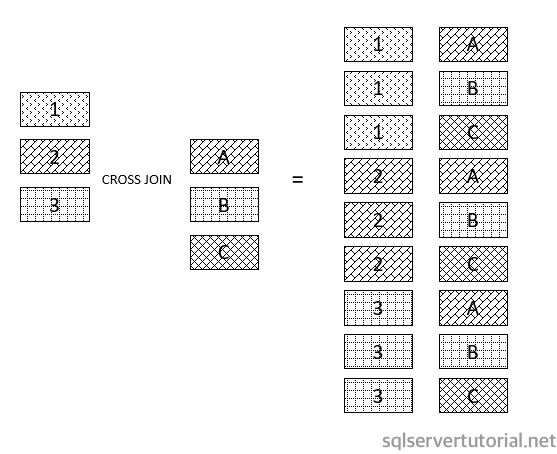
\includegraphics[width=0.7\linewidth]{images/worksheet_3_solution_1.png}
                \end{center}
            \end{itemize}
        \end{itemize}

        \item

        In this case, the resulting operation would have 7 attributes

        \bigskip

        (StarsIn.movieTitle, StarsIn.moveYear, StarsIn.starName,\\
        MovieStar.name, MovieStar.addresss, MovieStar.gender,\\
        MovieStar.birthDate)

        \bigskip

        with atrribute values of MovieStar returning null when StarsIn values
        are present, and vice versa

        \bigskip

        \underline{\textbf{Notes:}}

        \bigskip

        \begin{itemize}
            \item \textbf{Outerjoins:}
            \begin{itemize}
                \item Is equivalent form of Natural Join but with missing values in rows
                (i.e. dangling tuples) returning null

                \item \textbf{Syntax:} \textit{Relation 1} NATURAL FULL OUTER JOIN \textit{Relation 2}
                \item FULL OUTER JOIN VS NATURAL FULL OUTER JOIN
                \begin{itemize}
                    \item FULL OUTER JOIN
                    \begin{itemize}
                        \item Allows to explicitly define the keys for the join condition
                    \end{itemize}

                    \item NATURAL FULL OUTER JOIN
                    \begin{itemize}
                        \item Database engine chooses the keys based on common names
                    \end{itemize}
                \end{itemize}

                \bigskip

                \begin{center}
                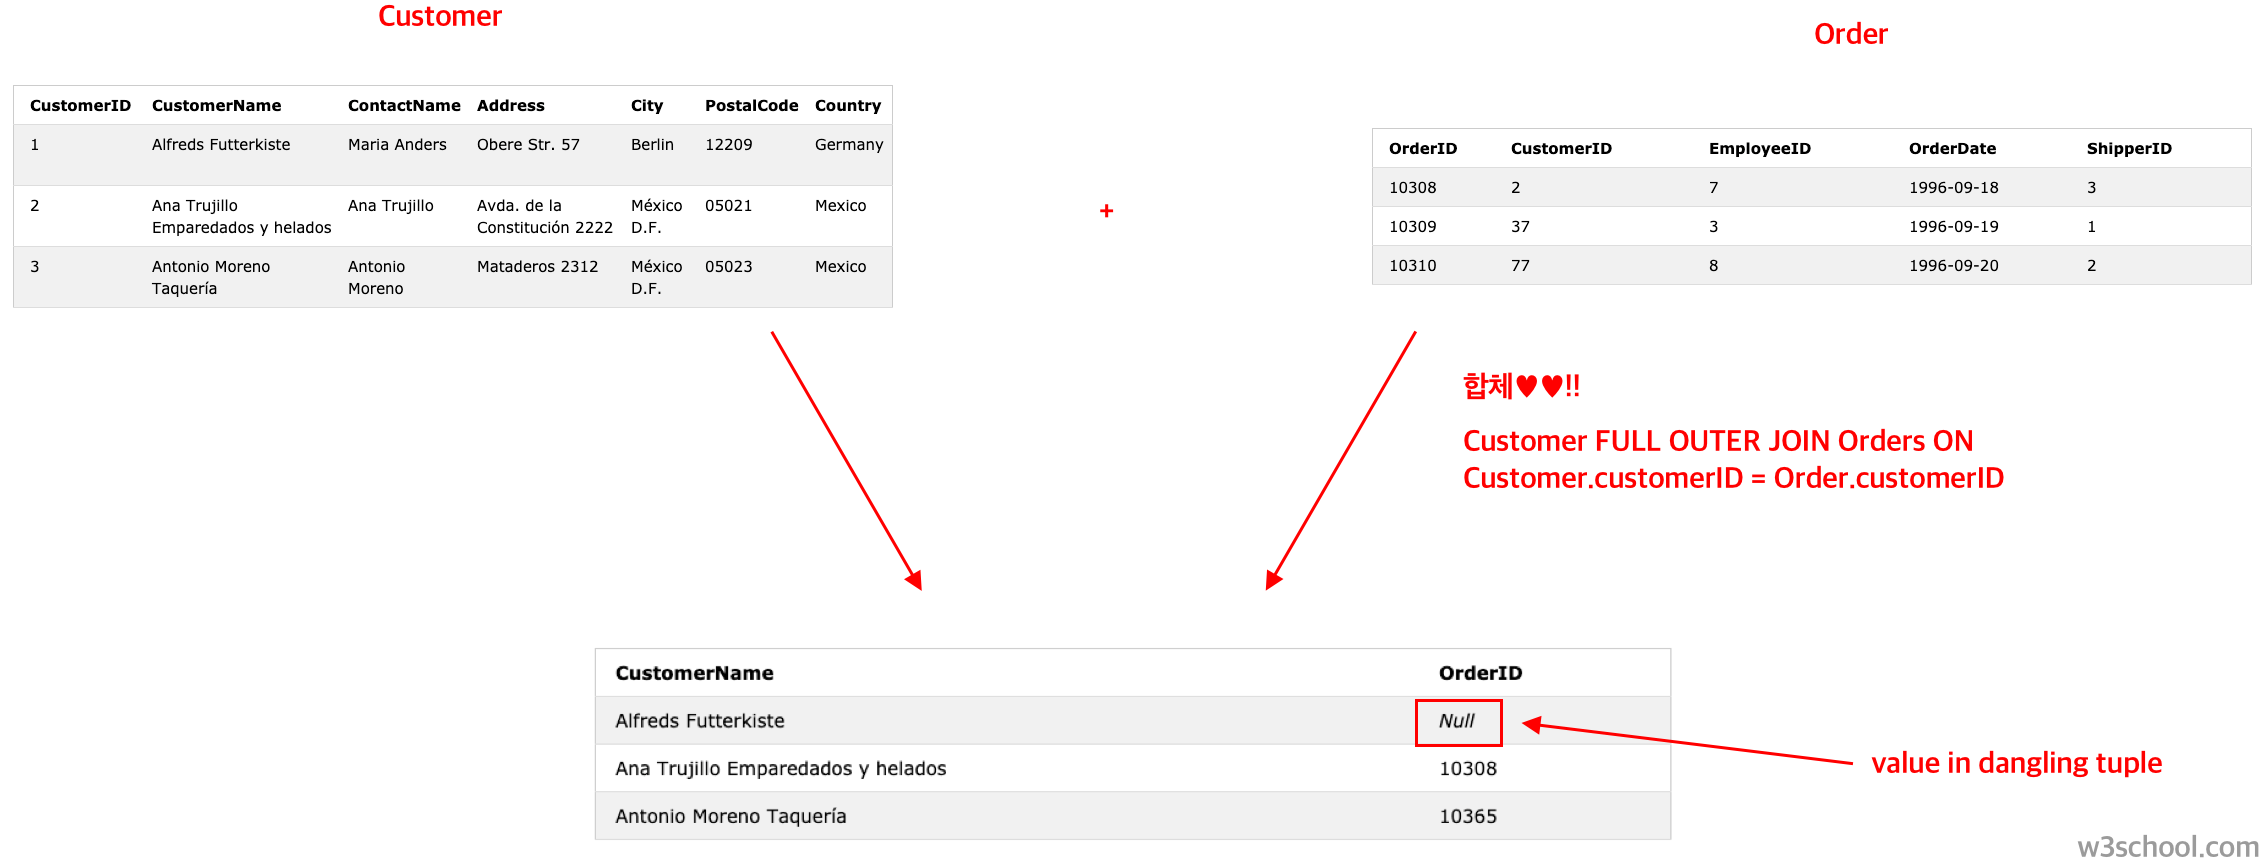
\includegraphics[width=\linewidth]{images/worksheet_3_solution_2.png}
                \end{center}

            \end{itemize}
        \end{itemize}

        \item

        In this case, the resulting operation would have 6 attributes

        \bigskip

        (StarsIn.movieTitle, StarsIn.moveYear,MovieStar.name, MovieStar.addresss,\\
        MovieStar.gender, MovieStar.birthDate)

        \bigskip

        and the atrribute values of MovieStar not present in StarsIn are padded with null,
        and vice versa


    \end{enumerate}

    \item

    \begin{lstlisting}[language=SQL]
    SELECT * FROM
    (SELECT * FROM PC NATURAL LEFT OUTER JOIN Product)
    NATURAL FULL OUTER JOIN
    (SELECT * FROM Laptop NATURAL LEFT OUTER JOIN Product)
    NATURAL FULL OUTER JOIN
    (SELECT p.model, p.color. p.type AS printType, p.price, pr.maker, pr.type FROM
    Printer AS p LEFT FULL OUTER JOIN
    Product AS pr ON Printer.model = Product.model)
    \end{lstlisting}

    \bigskip

    \begin{mdframed}
        \underline{\textbf{Correct Solution:}}

        \bigskip

    \begin{lstlisting}[language=SQL]
    SELECT * FROM
    (SELECT * FROM PC NATURAL LEFT OUTER JOIN Product)
    NATURAL FULL OUTER JOIN
    (SELECT * FROM Laptop NATURAL LEFT OUTER JOIN Product)
    NATURAL FULL OUTER JOIN
    (SELECT p.model, p.color. p.type AS printType, p.price, pr.maker, pr.type FROM
    Printer AS p LEFT OUTER JOIN                    // Corrected
    Product AS pr ON Printer.model = Product.model)
    \end{lstlisting}
    \end{mdframed}

    \item

    \begin{lstlisting}[language=SQL]
    SELECT * FROM Ships NATURAL LEFT OUTER JOIN Classes;
    \end{lstlisting}

    \item

    \begin{lstlisting}[language=SQL]
    SELECT * FROM Ships NATURAL FULL OUTER JOIN Classes
    WHERE ship = class;
    \end{lstlisting}

\end{enumerate}

\end{document}